\documentclass[aspectratio=169]{beamer}

\usetheme{Madrid}
\usecolortheme{seahorse}

\usepackage[utf8]{inputenc}
\usepackage[T1]{fontenc}
\usepackage[spanish]{babel}
\usepackage{tikz}
\usetikzlibrary{arrows.meta, positioning, shapes.geometric}
\usepackage{listings}
\usepackage{xcolor}
\usepackage{graphicx}

\lstdefinestyle{yaml}{
  basicstyle=\ttfamily\tiny,
  keywordstyle=\color{blue},
  commentstyle=\color{gray},
  numbers=none,
  breaklines=true,
  frame=single,
  backgroundcolor=\color{black!4}
}

\title{Observabilidad e Ingeniería de Tráfico}
\subtitle{Service Mesh con Istio sobre Bookinfo}
\author{Diego, Esteban, Emmanuel}
\date{\today}

\begin{document}

\begin{frame}
  \titlepage
\end{frame}

\begin{frame}{Agenda}
  \tableofcontents
\end{frame}

% ============================================================
\section{Stack de Observabilidad}
% ============================================================

\begin{frame}{Arquitectura del Mesh Bajo Observación}
  \centering
  \resizebox{!}{0.55\textheight}{%
  \begin{tikzpicture}[
      node distance=1.0cm and 1.4cm,
      svc/.style={draw, rounded corners, minimum width=2.2cm, minimum height=0.8cm, align=center, fill=blue!8},
      ext/.style={draw, rounded corners, minimum width=2.2cm, minimum height=0.8cm, align=center, fill=green!10}
    ]
    \node[ext] (gw) {Ingress\\Gateway};
    \node[svc, right=of gw] (pp) {productpage};
    \node[svc, above right=of pp] (det) {details};
    \node[svc, below right=of pp] (rev) {reviews\\(v1/v2/v3)};
    \node[svc, right=of rev] (rat) {ratings};

    \draw[-{Latex}] (gw) -- (pp);
    \draw[-{Latex}] (pp) -- (det);
    \draw[-{Latex}] (pp) -- (rev);
    \draw[-{Latex}] (rev) -- (rat);
  \end{tikzpicture}%
  }
  \vspace{0.3cm}
  \begin{center}
  \small Cada salto es una llamada de sidecar a sidecar de Envoy: Prometheus recolecta\\
  métricas, Jaeger recolecta spans, y Kiali renderiza el grafo en vivo a partir de ambos.
  \end{center}
\end{frame}

\begin{frame}{Kiali: Topología de Servicios}
  \begin{columns}
    \column{0.55\textwidth}
    \begin{itemize}
      \item Renderiza el grafo de tráfico en vivo a partir de datos de Prometheus, actualizado cada 15s.
      \item Muestra tasa de peticiones y \% de éxito por cada arista.
      \item Visualiza el enrutamiento ponderado (canary) y las aristas basadas en headers directamente sobre el grafo.
      \item La vista \textbf{Istio Config} lista cada CRD (VirtualService, DestinationRule, Gateway, PeerAuthentication, Telemetry) con su estado de validación.
    \end{itemize}
    \column{0.45\textwidth}
    \centering
    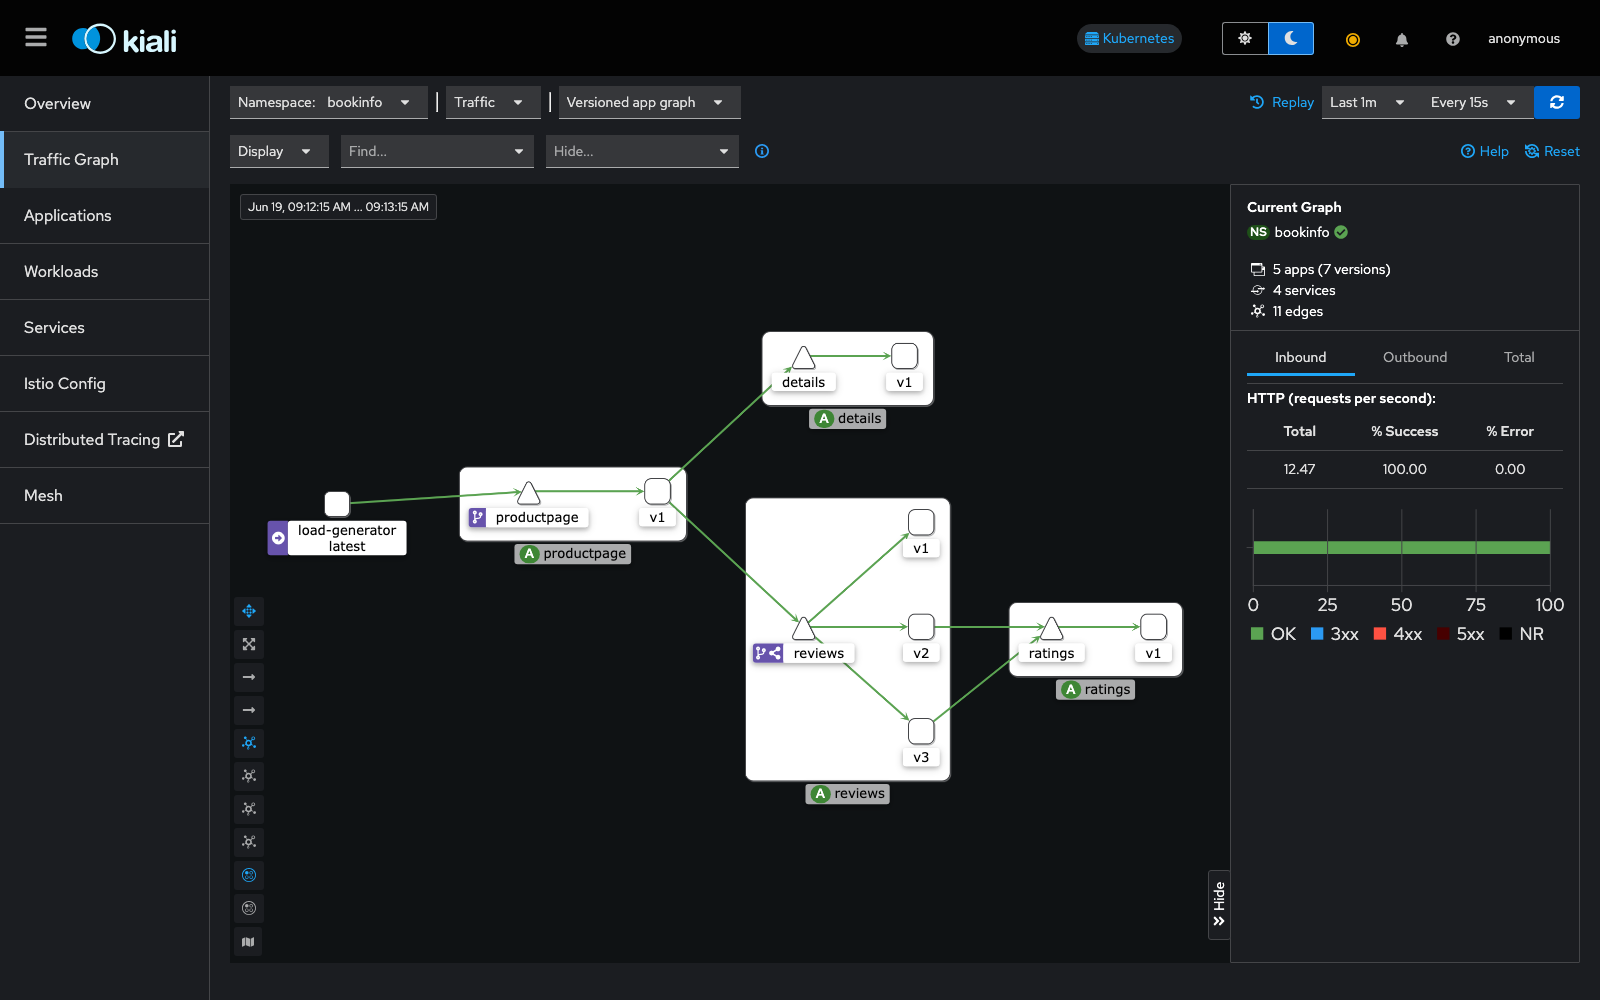
\includegraphics[width=\textwidth]{../docs/screenshots/routing/kiali_canary_topology.png}
  \end{columns}
\end{frame}

\begin{frame}{Grafana: Dashboards de Métricas}
  \begin{columns}
    \column{0.55\textwidth}
    \begin{itemize}
      \item \texttt{06-install-metrics.sh} instala Prometheus y un dashboard personalizado de \textbf{Bookinfo}.
      \item Tres paneles: tasa de peticiones por servicio, tasa de errores 5xx, y tasa de peticiones por versión de \texttt{reviews}.
      \item También están disponibles los dashboards estándar de Istio (Mesh, Service, Control Plane).
      \item Usado a lo largo del proyecto para evidenciar los splits de canary y los escenarios de inyección de fallas.
    \end{itemize}
    \column{0.45\textwidth}
    \centering
    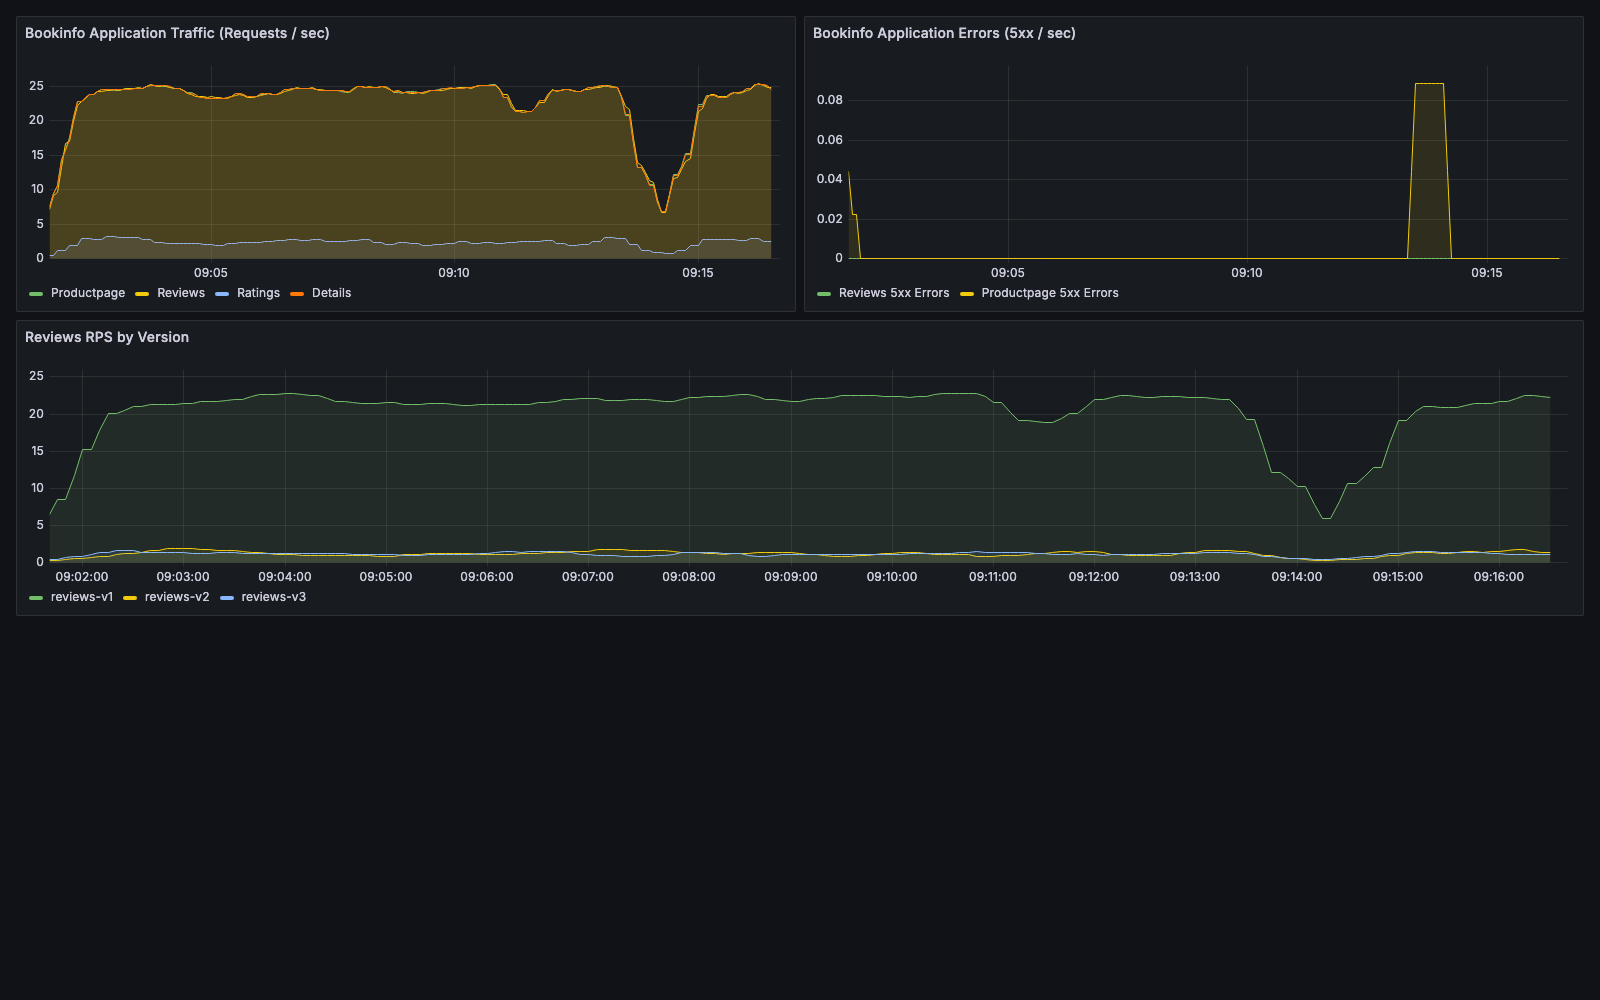
\includegraphics[width=\textwidth]{../docs/screenshots/routing/grafana_bookinfo_canary.png}
  \end{columns}
\end{frame}

\begin{frame}{Jaeger: Tracing Distribuido}
  \begin{columns}
    \column{0.55\textwidth}
    \begin{itemize}
      \item \texttt{07-install-tracing.sh} instala Jaeger (binario único) más un recurso \texttt{Telemetry} que fija el \textbf{sampling de trazas al 100\%} en \texttt{bookinfo} (frente al 1\% por defecto de Istio).
      \item Los servicios propagan los headers de tracing W3C/B3 de extremo a extremo, de modo que una sola traza abarca cada salto.
      \item Vista de búsqueda: cada petición que entra por \texttt{productpage}, abriéndose hacia \texttt{details} y \texttt{reviews}.
    \end{itemize}
    \column{0.45\textwidth}
    \centering
    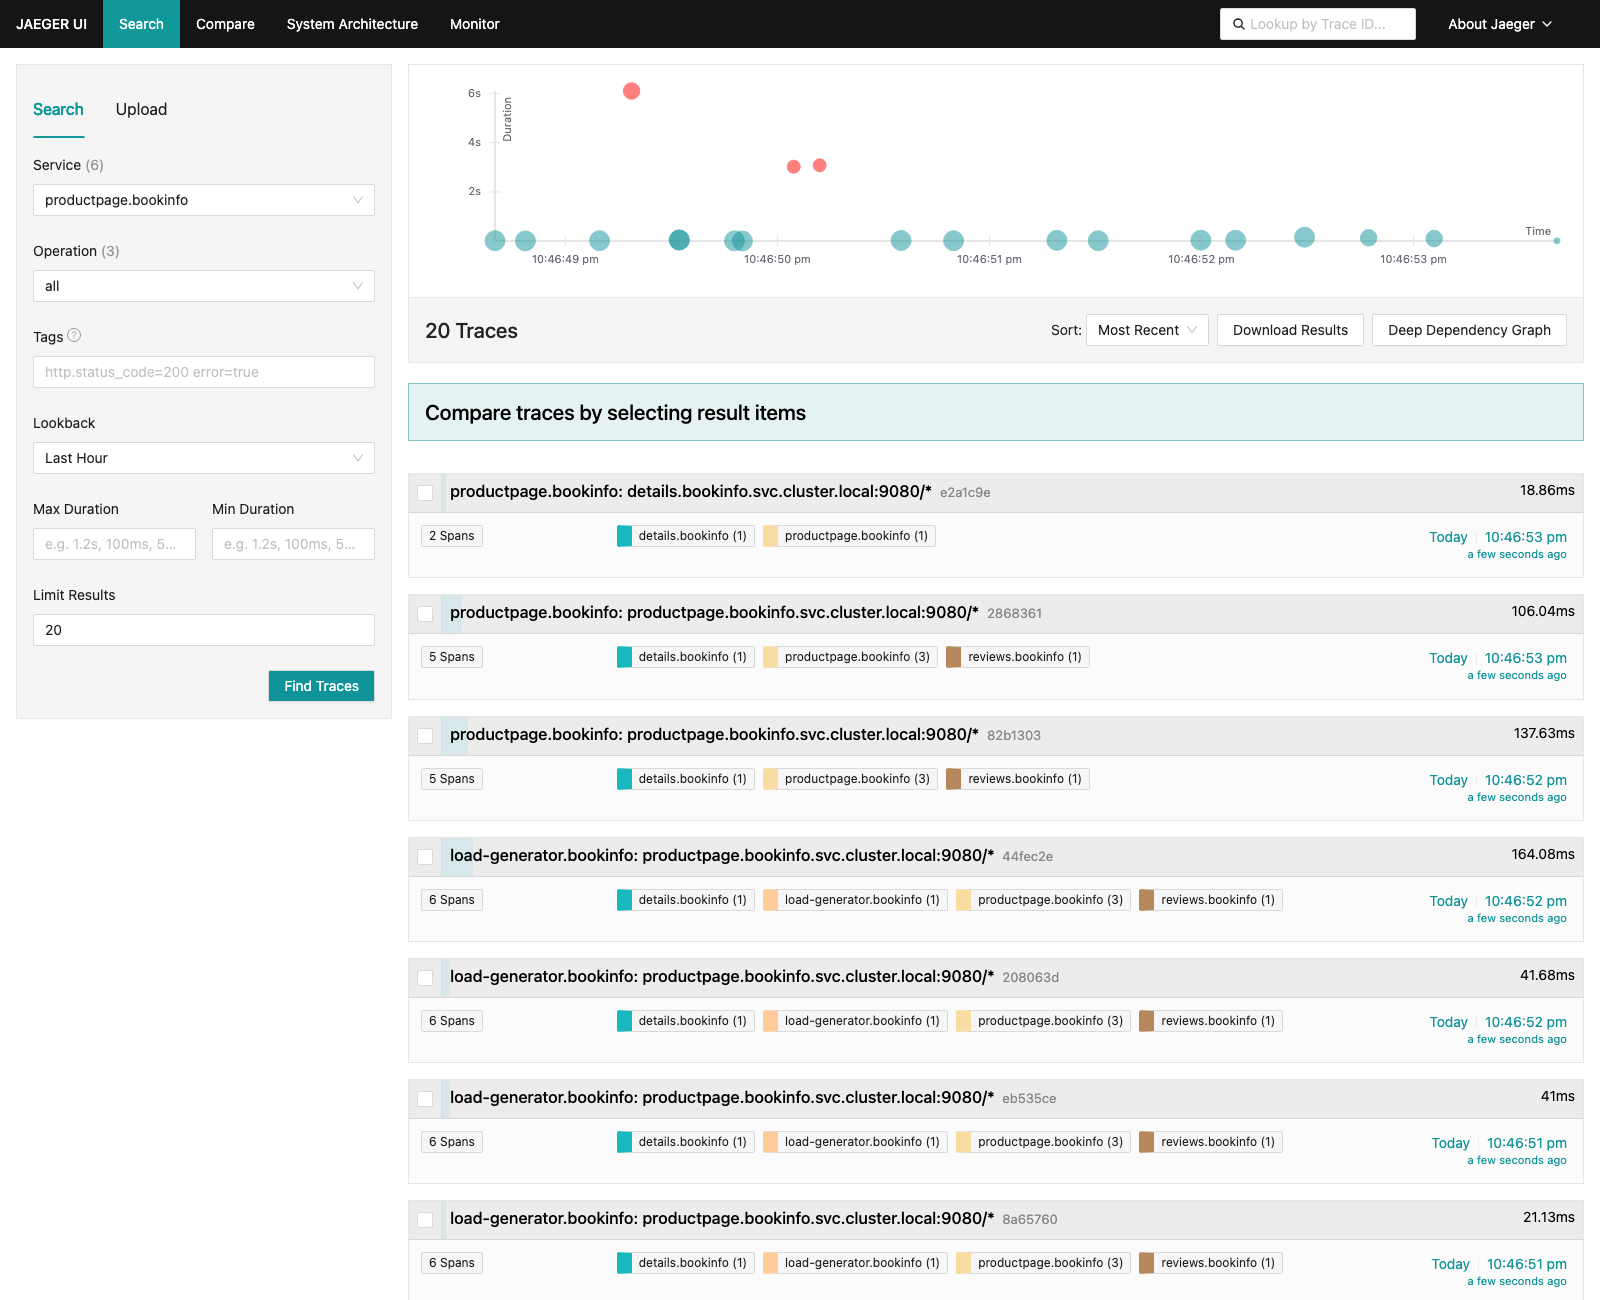
\includegraphics[width=\textwidth]{../docs/screenshots/tracing/jaeger_trace_list.png}
  \end{columns}
\end{frame}

\begin{frame}{Jaeger: Vista de Cascada (Waterfall)}
  \begin{columns}
    \column{0.55\textwidth}
    \begin{itemize}
      \item Árbol de llamadas completo: \texttt{load-generator $\to$ productpage $\to$ \{details, reviews $\to$ ratings\}}.
      \item 5 servicios, 12 spans, con tiempos por cada uno.
      \item Permite identificar exactamente qué llamada aguas abajo es lenta o está fallando --- por ejemplo, un span retrasado de \texttt{reviews $\to$ ratings} aparece de inmediato como un valor atípico.
    \end{itemize}
    \column{0.45\textwidth}
    \centering
    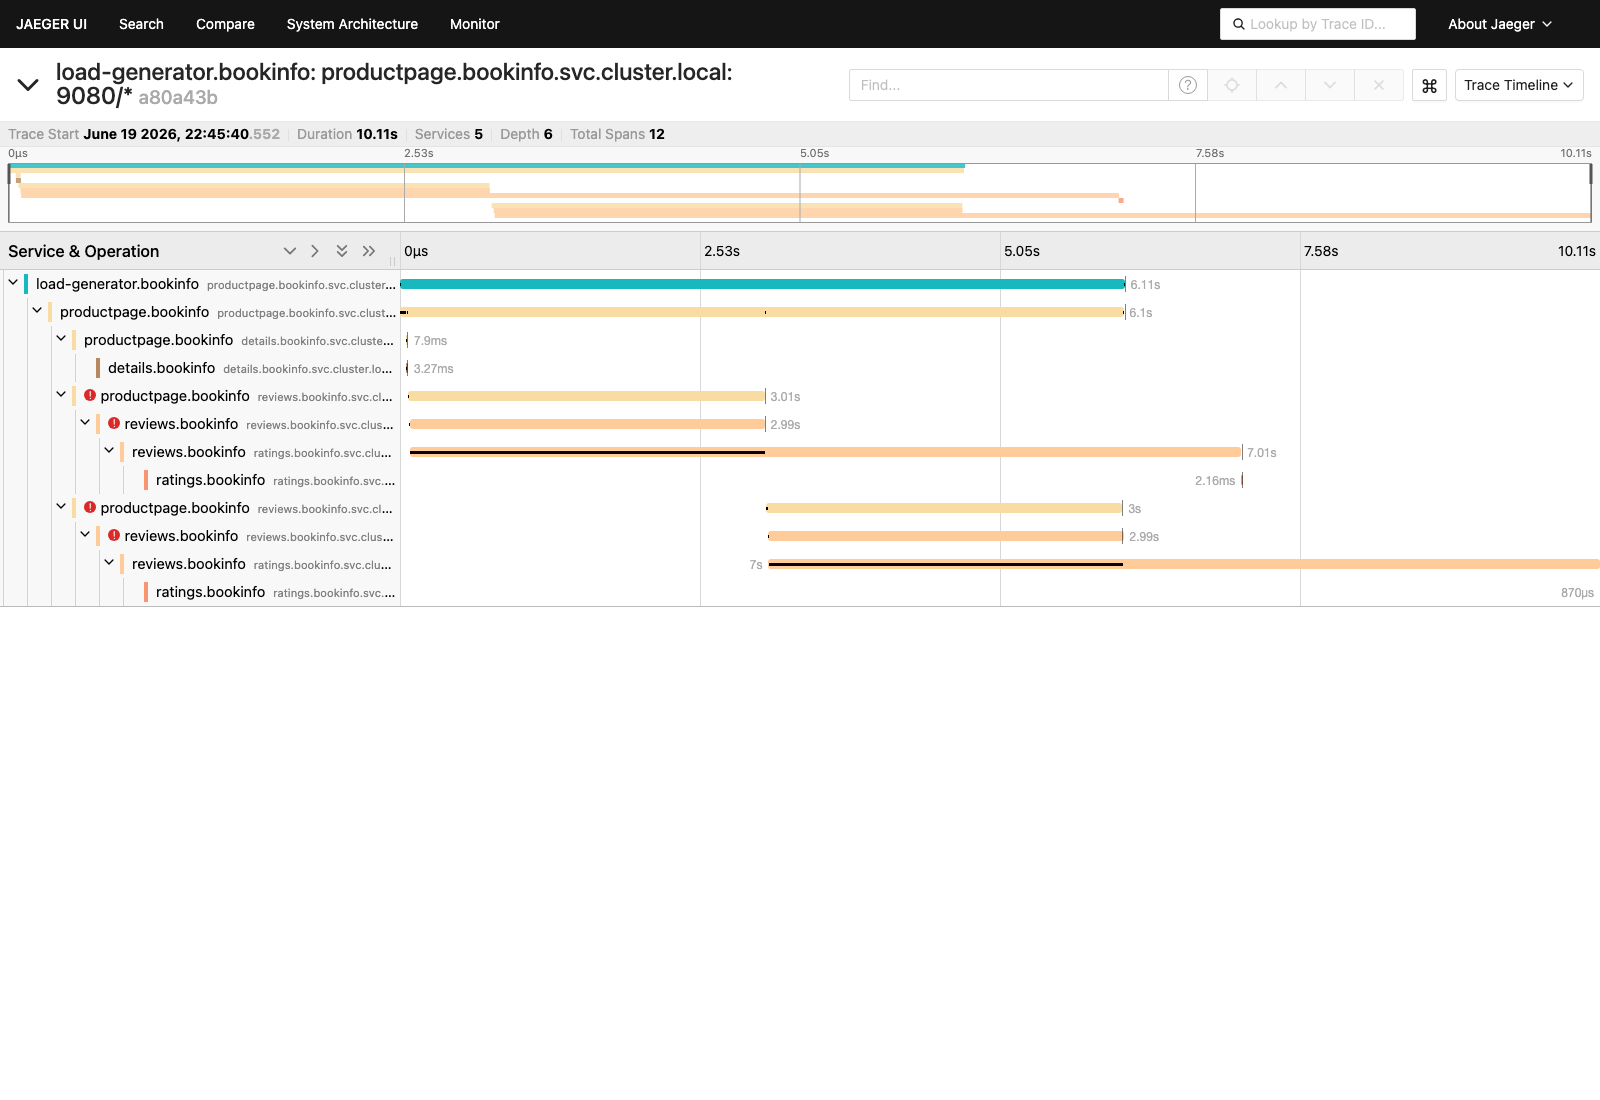
\includegraphics[width=\textwidth]{../docs/screenshots/tracing/jaeger_trace_detail.png}
  \end{columns}
\end{frame}

% ============================================================
\section{Ingeniería de Tráfico}
% ============================================================

\begin{frame}{Ingeniería de Tráfico: Visión General}
  \begin{itemize}
    \item Objetivo: controlar cómo se distribuyen las peticiones a \texttt{reviews} entre \texttt{v1}/\texttt{v2}/\texttt{v3} sin tocar el código de la aplicación.
    \item Dos mecanismos complementarios, ambos expresados como recursos \texttt{VirtualService} de Istio:
    \begin{enumerate}
      \item \textbf{Canary release} --- split de tráfico ponderado.
      \item \textbf{Enrutamiento basado en headers} --- enrutamiento determinista para un usuario específico.
    \end{enumerate}
    \item Combinados en un único \texttt{VirtualService} con reglas de match HTTP ordenadas por prioridad.
  \end{itemize}
\end{frame}

\begin{frame}[fragile]{Canary Release: Split 90/5/5}
  \texttt{networking/virtual-service-canary.yaml}
  \begin{lstlisting}[style=yaml]
apiVersion: networking.istio.io/v1
kind: VirtualService
metadata:
  name: reviews-canary
spec:
  hosts: [reviews]
  http:
  - route:
    - destination: {host: reviews, subset: v1}
      weight: 90
    - destination: {host: reviews, subset: v2}
      weight: 5
    - destination: {host: reviews, subset: v3}
      weight: 5
  \end{lstlisting}
  \texttt{scripts/10-verify-canary.sh} muestrea 100 peticiones y confirma que el
  ratio v2+v3 cae dentro de $10\% \pm 5\%$.
\end{frame}

\begin{frame}[fragile]{Enrutamiento Basado en Headers}
  \texttt{networking/combined-virtual-service.yaml} --- orden de prioridad:
  \begin{enumerate}
    \item Header \texttt{end-user: jason} $\to$ 100\% hacia \texttt{reviews-v2}.
    \item Todo lo demás $\to$ cae en el split canary 90/5/5.
  \end{enumerate}
  \begin{lstlisting}[style=yaml]
http:
  - name: header-based-routing
    match:
    - headers: {end-user: {exact: "jason"}}
    route:
    - destination: {host: reviews, subset: v2}
      weight: 100
  - name: canary-default-routing
    route:
    - destination: {host: reviews, subset: v1}
      weight: 90
    - destination: {host: reviews, subset: v2}
      weight: 5
    - destination: {host: reviews, subset: v3}
      weight: 5
  \end{lstlisting}
\end{frame}

\begin{frame}{Camino de Decisión del Enrutamiento}
  \centering
  \resizebox{!}{0.55\textheight}{%
  \begin{tikzpicture}[
      node distance=0.8cm and 1.2cm,
      box/.style={draw, rounded corners, minimum width=3.2cm, minimum height=0.8cm, align=center},
      dec/.style={draw, diamond, aspect=2.2, minimum width=3.2cm, align=center, fill=yellow!15}
    ]
    \node[box, fill=blue!8] (req) {Petición entrante\\a \texttt{reviews}};
    \node[dec, below=of req] (chk) {\texttt{end-user:}\\\texttt{jason}?};
    \node[box, fill=green!10, below left=0.9cm and 0.2cm of chk] (v2) {100\% $\to$ reviews-v2};
    \node[box, fill=orange!10, below right=0.9cm and 0.2cm of chk] (canary) {90\% v1 / 5\% v2 / 5\% v3};

    \draw[-{Latex}] (req) -- (chk);
    \draw[-{Latex}] (chk) -- node[left]{sí} (v2);
    \draw[-{Latex}] (chk) -- node[right]{no} (canary);
  \end{tikzpicture}%
  }
  \vspace{0.3cm}
  \texttt{scripts/11-test-header-routing.sh} confirma ambos caminos: una petición
  anónima recibe cualquier versión válida, una petición de \texttt{jason} siempre recibe \texttt{v2}.
\end{frame}

\begin{frame}{Efecto Observado: Split de Tráfico en Kiali}
  \centering
  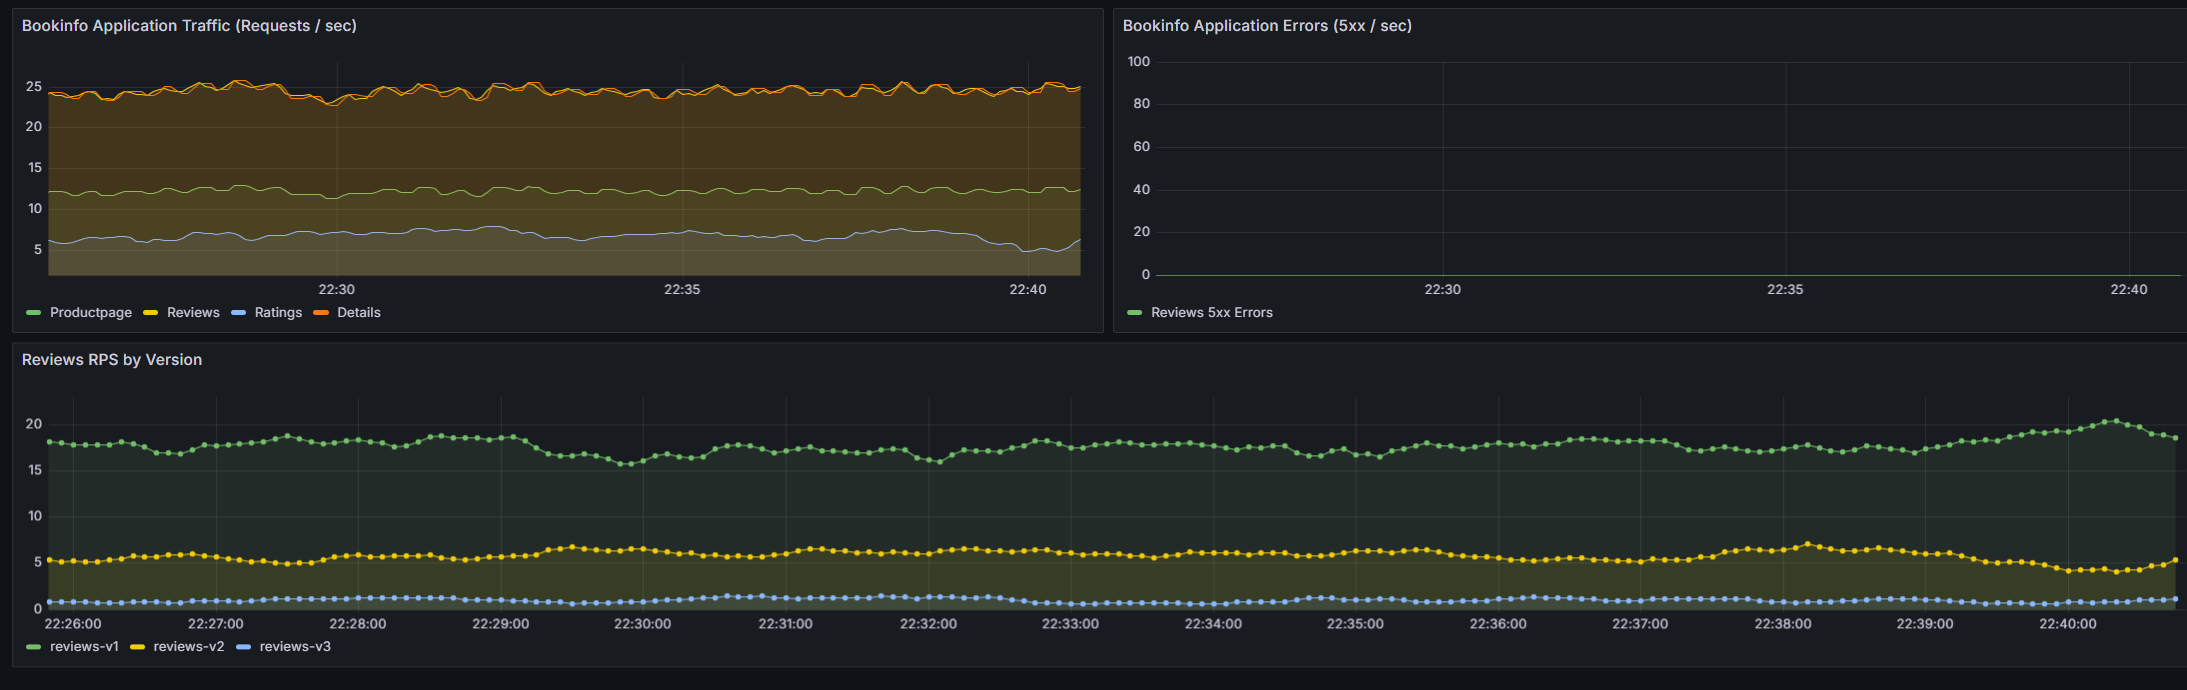
\includegraphics[width=0.7\textwidth]{../docs/screenshots/routing/kiali_traffic_split.png}
  \begin{center}
  \small Kiali renderiza tanto las aristas ponderadas hacia v1/v2/v3 como la
  arista basada en header hacia v2, bajo carga.
  \end{center}
\end{frame}

% ============================================================
\section{Demostración en Vivo}
% ============================================================

\begin{frame}{Demostración en Vivo}
  \begin{enumerate}
    \item Cluster, Istio, Bookinfo, métricas y tracing ya en ejecución
          (\texttt{scripts/run-all.sh}, líneas 1--37).
    \item Aplicar el \texttt{VirtualService} de \textbf{canary} y ejecutar
          \texttt{10-verify-canary.sh}.
    \item Aplicar el \texttt{VirtualService} \textbf{combinado basado en headers} y ejecutar
          \texttt{11-test-header-routing.sh}.
    \item Observar el efecto en vivo en \textbf{Kiali}, \textbf{Grafana} y \textbf{Jaeger}.
  \end{enumerate}
  \vspace{0.5cm}
  \centering
  \textit{Sin más diapositivas --- pasamos a la terminal y al navegador.}
\end{frame}

\begin{frame}{Gracias}
  \centering
  \Large ¿Preguntas?
\end{frame}

\end{document}
